\documentclass{math201}

\usepackage[backref]{hyperref} 
\hypersetup{hidelinks}
\usepackage{bookmark}

% =============================================
% Part 0 信息
% =============================================

\mathsetup{
  % 学生姓名
  student = {},
  % 学号
  student-id = {},
  % 院系
  experiment = {DSP 2812控制板的硬件设计},
  % 专业年级
  discipline = {集成电路设计与集成系统},
  % 日期
  date = {\today},
}

\begin{document}

% =============================================
% Part 1  封面
% =============================================

\makecover

% =============================================
% Part 2 主文档
% =============================================

\section{实验内容}

通过DSP的通用输入输出多路复合器GPIO来控制LED灯的闪烁

\section{实验步骤}

\begin{figure}[H]  
    \centering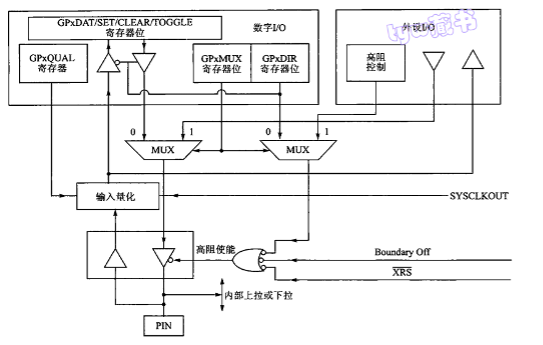
\includegraphics[width=0.8\linewidth]{Picture1.jpg}  
    \caption{从以下6个方面详细分析,要求截图、配合文字说明}     
\end{figure}

\section{TMS320X2812最小系统}

主要由TMS320X2812芯片、晶振和电源电 路以及电容、电阻电感等少量器件构成。还需要JTAG下载接口电路。

TMS320F2812 176 引脚 PGF LQFP

\subsection{电源电路}

电源电路使用的电源管理芯片包括:LM2596-5, TPS75733, TPS76801。
这些芯片可以提供不同的输出电压,满足DSP芯片和其他外设的电源需求。
例如,LM2596-5可以提供5V输出,用于给DSP芯片的I/O端口供电;
TPS75733可以提供3.3V输出,用于给DSP芯片的内核和外部存储器供电;
TPS76801可以提供1.8V输出,用于给DSP芯片的模拟外设供电。

\begin{figure}[H]  
  \centering\includegraphics[width=0.8\linewidth]{EX2\_TPS75733\_1.png}  
  \caption{TPS75733}     
\end{figure}

\begin{figure}[H]  
  \centering\includegraphics[width=0.8\linewidth]{EX2\_TPS76801\_1.png}  
  \caption{TPS76801}     
\end{figure}

\begin{figure}[H]  
  \centering\includegraphics[width=0.8\linewidth]{EX2\_LM2596-5\_1.png}  
  \caption{LM2596-5}     
\end{figure}

\subsection{复位电路}

包含上电复位、手动复位。按下K1复位键,XRS输出低电平,复位DSP芯片。保护电路中使用CM1215。

\subsection{时钟电路、JTAG下载电路}

时钟电路使用了一个外部晶振作为时钟源,晶振的频率为30MHz。
时钟信号经过一个反相器后输入到TMS320F2812芯片的X1引脚。
TMS320F2812芯片内部有一个可编程时钟发生器(PLL),可以将外部时钟信号倍频到150MHz。

\begin{figure}[H]  
  \centering\includegraphics[width=0.8\linewidth]{EX2\_reset\_1.png}  
  \caption{reset}     
\end{figure}

\begin{figure}[H]  
  \centering\includegraphics[width=0.8\linewidth]{EX2\_OSC\_1.png}  
  \caption{OSC}     
\end{figure}

JTAG下载电路使用了一个标准的14针JTAG接口。
JTAG接口可以连接到PC机上的仿真器或下载器,通过JTAG协议实现对TMS320F2812芯片的编程、调试和测试。
JTAG下载电路还使用了一些上拉电阻和保护二极管来保证信号的稳定和安全。

\section{显示电路}

\subsection{流水灯电路}

流水灯电路是一种利用 LED 发光二极管实现动态显示效果的电路,
它可以用来测试控制板的 GPIO 引脚功能和编程能力。
TMS320X2812 的控制板上有 8 个 LED 灯,分别连接到 F2812 的 GPIOA0~GPIOA7 引脚,
通过编程控制这些引脚的高低电平,就可以实现流水灯的效果。

\subsection{数码管电路}

TMS320F2812使用6个共阳极14脚数码管,型号为CL3661BH。

\begin{figure}[H]  
  \centering\includegraphics[width=0.8\linewidth]{EX2\_CL3661BH\_1.png}  
  \caption{CL3661BH}     
\end{figure}

数码管电路是一种利用数码管显示数字或字符的电路,它可以用来显示控制板的运行状态或数据信息。
TMS320X2812 的控制板上有 6 个共阳极14脚数码管,
分别连接到 F2812 的 GPIOB0~GPIOB5 引脚(位选)和 GPIOC0~GPIOC7 引脚(段选),
通过编程控制这些引脚的高低电平,就可以实现数码管的显示。

\section{外扩并行存储器}

通过XINTF接口来外扩存储器
三大总线:地址总线、数据总线、控制总线
地址总线:XA[0..18]
数据总线:XD[0..15]
控制总线: XZCS0/1, XZCS2, XZCS6/7, XRD, XWE, XR/W, XHOLD, XHOLDA, XMP/MC

\subsection{外扩RAM电路}

外扩RAM512K×16位,分别连接到XINTF的区域0和区域1。
每片芯片有19位地址线和16位数据线,所以可以存储256K×16位的数据。
芯片的地址线A[0…18]分别连接到XA[0…18],数据线DQ[0…15]分别连接到XD[0…15]。
芯片的片选信号CE1和CE2分别连接到XZCS6/7,输出使能信号OE连接到XRDL,写使能信号WE连接到XWEL。
芯片的时钟信号CLK和字节写使能信号BHE和BLE都接地,不使用。

\begin{figure}[H]  
  \centering\includegraphics[width=0.8\linewidth]{EX2\_RAM512\_1.png}  
  \caption{RAM512}     
\end{figure}

\section{A/D采样模块}

这块控制板有 16 个模拟输入信号引脚,分别对应 TMS320X2812 的 ADCINA0~ADCINA15。
这些引脚可以用来采集外部的模拟信号,如温度、电压、电流等。

采样电路是指将模拟信号转换为数字信号的电路,通常由采样保持器、模数转换器和时钟信号组成。
在这块控制板上,采样保持器和模数转换器都集成在 TMS320X2812 的内部,
而时钟信号可以由外部提供,也可以由内部的定时器产生。

\begin{figure}[H]  
  \centering\includegraphics[width=0.8\linewidth]{EX2\_CYDL\_1.png}  
  \caption{采样电路}     
\end{figure}

静电保护电路是指用来防止静电对电路造成损坏的电路,通常由二极管、晶体管或专用的静电保护芯片组成。
在这块控制板上,静电保护电路使用了 CM1215 这款芯片,它可以提供高达 ±15kV 的接触放电和 ±25kV 的空气放电的保护。
CM1215 芯片与 16 个模拟输入信号引脚相连,可以有效地吸收静电并将其释放到地线上。

\section{PWM电路的电平转换}

PWM波形的高电压是3.3V,实际工业控制中,驱动电压往往是5V。
为了实现PWM信号的电平转换,需要使用一种双向数据传输器,即74AHCT2451。

74AHCT2451是一种8位双向总线收发器,具有三态输出。
该器件具有输出使能(OE)和发送/接收(DIR)两个控制信号,用于控制数据传输的方向和输出状态。
当OE为高电平时,输出处于高阻态;
当DIR为高电平时,数据从A端口传输到B端口;
当DIR为低电平时,数据从B端口传输到A端口。输入具有过压容限性,可以接受高达5.5V的输入电压。

74AHCT2451的工作电压范围是2.0V到5.5V,输入逻辑电平为TTL水平,输出驱动能力为±8mA,
传输延迟时间为3.5ns,最大工作频率为60MHz。
该器件可以在-40°C到+125°C的温度范围内工作。

PWM信号的电平转换电路如图所示:

\begin{figure}[H]  
  \centering\includegraphics[width=0.8\linewidth]{EX2\_PWM\_1.png}  
  \caption{PWM信号的电平转换电路}     
\end{figure}

在这个电路中,74AHCT2451的A端口接收来自TMS320X28122的PWM信号,B端口输出转换后的PWM信号。
OE和DIR都接地,使得数据从A端口传输到B端口,并且输出始终有效。
VCC接5V电源,GND接地。
由于74AHCT2451的输入具有过压容限性,所以不需要在A端口和TMS320X28122之间加任何保护元件。
这样,就可以实现PWM信号从3.3V转换到5V的功能,从而驱动更高电压的负载。

\section{串行通信接口电路}

\subsection{SCI通信电路}

SCI(串行通信接口)是一种用于异步串行数据传输的通信协议。
TMS320X2812芯片内部集成了两个SCI模块,分别为SCI-A和SCI-B1。
这两个模块可以独立工作,也可以同时工作,实现双通道的串行通信1。

SCI通信电路的主要功能是将TMS320X2812芯片的逻辑信号转换为RS-485或RS-422标准的差分信号,
以提高抗干扰能力和传输距离。为了实现这一功能,需要使用以下几种芯片:

ISO3082:这是一种隔离式的半双工差分线收发器,用于TIA/EIA 485/422应用2。
它可以提供2500 VRMS的隔离电压,以及高达20 Mbps的信号速率2。
它还具有ESD、EFT和雷击保护功能2。

SM712:这是一种非对称的TVS二极管阵列,用于保护RS-485应用免受静电放电(ESD)、
电气快速瞬变(EFT)和雷击引起的浪涌3。它可以吸收高达30 kV的重复ESD冲击,
以及高达19 A的8/20us浪涌电流3。

B82790:这是一种信号线共模电感器,用于抑制共模噪声和提高通信质量4。
它具有高达1.8 kΩ的共模阻抗,以及高达500 mA的额定电流4。

SCI通信电路的原理图如下:

\begin{figure}[H]  
  \centering\includegraphics[width=0.8\linewidth]{EX2\_SCI\_1.png}  
  \caption{SCI通信电路的原理图}     
\end{figure}

\subsection{CAN电路}

CAN(控制器局域网)是一种用于实时控制系统的串行通信协议。
它具有高速、可靠、多主机、多任务等特点。
TMS320X2812芯片内部集成了一个CAN模块,支持CAN 2.0A和CAN 2.0B标准1。
CAN电路的主要功能是将TMS320X2812芯片的逻辑信号转换为符合ISO 11898标准的差分信号,以实现高速、长距离、多节点的网络通信。为了实现这一功能,需要使用以下几种芯片:

XCANTXDA和XCANRXDA:这是两个专用于TMS320X2812芯片的CAN驱动器和接收器芯片5。它们可以提供3.3 V或5 V的逻辑电平转换,以及热关断保护、过压保护和短路保护等功能5。

1050:这是一种隔离式的全双工差分线收发器,用于ISO 11898-2应用6。它可以提供5600 VRMS的隔离电压,以及高达1 Mbps的信号速率6。它还具有ESD、EFT和雷击保护功能。

SM712:这是一种非对称的TVS二极管阵列,用于保护CAN总线免受静电放电(ESD)、电气快速瞬变(EFT)和雷击引起的浪涌3。它可以吸收高达30 kV的重复ESD冲击,以及高达19 A的8/20us浪涌电流3。

B82790:这是一种信号线共模电感器,用于抑制共模噪声和提高通信质量4。它具有高达1.8 kΩ的共模阻抗,以及高达500 mA的额定电流4。

CAN电路的原理图如下:

\begin{figure}[H]  
  \centering\includegraphics[width=0.8\linewidth]{EX2\_CAN\_1.png}  
  \caption{CAN电路的原理图}     
\end{figure}

\subsection{SPI 、IIC电路}

SPI(串行外设接口)和IIC(内部总线)是两种常用的串行通信协议。它们可以用于连接TMS320X2812芯片和各种外部设备,如实时时钟、扩展存储器等。TMS320X2812芯片内部集成了一个SPI模块和一个IIC模块,支持主机或从机模式1。

SPI和IIC电路的主要功能是提供适合不同设备的接口电平和信号时序。为了实现这一功能,需要使用以下几种芯片:

SPI\_Interface:这是一个引出接口,用于连接TMS320X2812芯片的SPI端口和外部设备的SPI端口7。它可以提供3.3 V或5 V的逻辑电平转换,以及过压保护、短路保护等功能7。

RX-8025SA:这是一种带有IIC总线接口的实时时钟模块8。它内置了32.768 kHz的晶体振荡器,并经过高精度校准(±5×10 -6 / Ta=+25°C)。它还具有各种检测功能、双重闹钟功能、周期性中断功能等8。

扩展串行EEPROM:这是一种使用IIC总线接口的非易失性存储器芯片,用于存储TMS320X2812芯片的配置数据或用户数据10。它具有低功耗、高速度、大容量等特点10。

SPI和IIC电路的原理图如下:

\begin{figure}[H]  
  \centering\includegraphics[width=0.8\linewidth]{EX2\_SPI\_1.jpg}  
  \caption{SPI电路的原理图}     
\end{figure}

\begin{figure}[H]  
  \centering\includegraphics[width=0.8\linewidth]{EX2\_IIC\_1.jpg}  
  \caption{IIC电路的原理图}     
\end{figure}

\section{实验小结}

\end{document}
